\documentclass{article}

\usepackage{graphicx}
\usepackage{hyperref}

\title{Smart Lighting System}
\author{Simone Leoni \\
\footnotesize {\tt simone.leoni@studenti.unimi.it}}
\date{}

\begin{document}
	\maketitle
	
	\section{Introduzione}
	La continua evoluzione delle tecnonlogie attuali e, l'inizio della progettazione delle \textit{smartcity}, ha reso necessaria l'evoluzione di tutti i dispositivi all'interno del contesto urbano.
	Attualmente, tra le varie evoluzioni proposte, una tipologia di dispositivi che ha visto un grosso sviluppo verso una versione
	\textit{smart} sono gli impianti di illuminazione.
	
	\noindent Lo stato dell'arte attuale vede sistemi di illuminazione che presentano:
	\begin{itemize}
		\item Controllo automatico del livello di luce emessa in base alla luminosit\`a ambientale.
		\item Incremento dell'intensit\`a luminosa al passaggio di individui nelle vicinanze.
		\item Controllo remoto dello stato di funzionamento, accensione e spegnimento dei singoli dispositivi.
	\end{itemize}
	Tutte queste caratteristiche permettono di avere una gestione pi\`u efficiente dal punto di vista energetico dell'illuminazione
	urbana, non risulta infatti necessario mantenere livelli di iluuminazione elevate nelle aree poco trafficate.
	La possibilit\`a inoltre di conoscere lo stato di funzionamento dei singoli dispostivi permette una manutenzione pi\`u efficiente.
	
	\noindent La versione del progetto realizzato prevede una serie di feature presenti anche nello stato dell'arte attuale aggiungendo alcune piccole modifiche per una migliore integrazione all'interno delle \textit{smart city} e un tentativo di migliorare il contesto di sicurezza urbana.
	Il sistema realizzato prevede le seguenti feature:
	\begin{itemize}
		\item Controllo del sistema di illuminazione da remoto con accensione e spegnimento delle varie fetaure tramite rete LoRa.
		\item Livello di illuminazione controllato automaticamente in base al livello di luce ambientale.
		\item Incremento dell'intensit\`a luminosa al passaggio di individui nei pressi del sistema.
		\item \textit{Panic button} per la segnalazione di eventuali situazioni di emergenza alle forze dell'ordine e emissione di un segnale sonoro per attirare l'attenzione dei passanti.
	\end{itemize}
	L'aggiunta di un \textit{panic button}, come evidenziato in precedenza \`e stato pensato per migliorare il livello di sicurezza urbana. Grazie a questo elemento, infatti, adeguatamente integrato con telecamere di sicurezza, sarebbe possibile ottenere
	una sengalazione tempestiva delle sitauzioni di emergenza aggiungendo inoltre la possibilit\`a di attirare l'attenzione dei
	passanti e cercare quindi di sventare le situazioni di pericolo e/o emergenza anche tramite l'aiuto di cittadini presenti in loco.
	
	\section{Hardware utilizzato}
	Il sistema realizzato presenta diverse componenti hardware:
	\begin{itemize}
		\item Scheda di sviluppo STM32F411e-disco: essendo il progetto un proof of concept é stata utilizzata una development board commerciale, per poter rendere il progetto in questione, un possibile dispositivo atto alla vendita sarebbe necessaria la realizzazione di un PCB custom contenente tutto l'hardware necessario e una forma consona alla dissipazione del calore.
		\item Matrice led CharlieWing: elemento utilizzato per generare l'illuminazione necessaria. La matrice utilizzata viene comandata tramite \textit{i2c} all'indirizzo \texttt{0x74}.
		\item Scheda di sviluppo Raspberrypi Pico: per realizzare la comunicazione wireless senza aggiungere un eccessivo overhead sull'MCU \`e stato introdotto un coprocessore che gestisse autonomamente la comunicazione wireless tramite LoRa. 	Per effettuare la comunicazione tramite LoRa viene utilizzato un dispositivo \href{https://www.waveshare.com/wiki/Pico-LoRa-SX1262}{WaveShare LoRa Shield} basato su SX1262.
		\item Sensori di movimento SR602: per poter aumentare l'intensit\`a luminosa al passaggio di cittadini nei pressi del sistema di illumincazione sono stati introdotit dei sensori di movimento per rilevarne la presenza.
		\item Fotoresistore: la presenza di un foto resistore permette di rilevare il livello di luminosit\`a ambientale e regolare l'intensit\`a della luce emessa conseguentemente.
		\item Panic button: la presenza di questo bottone \`e intesa per la segnalazione delle situazioni di emergenza.
		\item Panic buzzer attivo: utilizzato per l'emissione di un segnale sonore atto ad attirare l'attenzione in situazioni di emergenza.
	\end{itemize}
	In Figura \ref{img:hw} \`e evidenziata la schematica di collegamento dei dispositivi hardware coinvolti.
	
	\begin{figure}[ht]
		\centering
		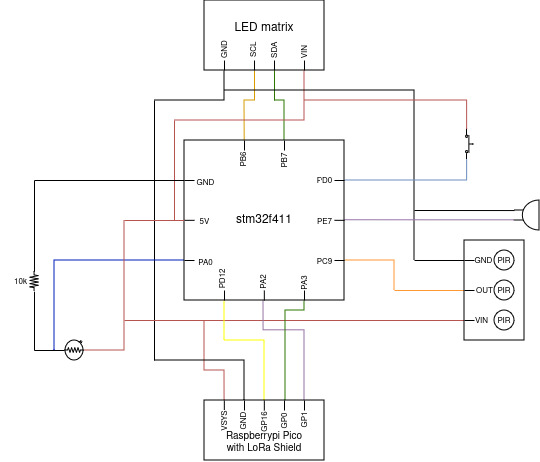
\includegraphics[scale=0.50]{./images/Hardware_schematic.jpg}
		\caption{Schematica di collegamento dei dispositivi hardware}
		\label{img:hw}
	\end{figure}
	\newpage
	
	\section{Architettura Software}
	Dal punto di vista software \`e necessario distinguire due diverse architetture: l'architettura dal punto di vista dell'MCU e l'architettura dal punto di vista del coprocessore wireless.
	
	\subsection{MCU}
	Il software presente sull'MCU, stm32f411, responsabile del funzionamento generale del sistema, risulta essere suddiviso in tre elementi principali: un componente di comunicazione con il coprocessore wireless, un componente per la gestione dell'illuminazione e una parte dedicata alle segnalazione di emergenza.
	Pur essendo tre le componenti del sistema il software risulta essere suddiviso in quattro moduli, oltre ai tre moduli precedentemente indicati, infatti, \`e presente un modulo di gestione dei sensori. Questo modulo pu\`o essere considerato parte della componente atta alla gestione dell'illuminazione essendo l'unico modulo che ne sfrutta il funzionamento.
	
	\subsubsection{Modulo Light}
	\begin{figure}[ht]
		\centering
		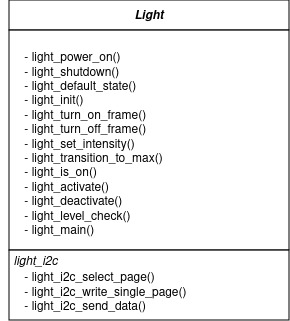
\includegraphics[scale=0.40]{./images/Light.jpg}
		\caption{Modulo Lights}
		\label{img:lights}
	\end{figure}
	Il modulo \textit{Light}, come si pu\`o intuire dal nome, risulta essere il modulo atto alla gestione del sistema di illuminazione. 
	Come si pu\`o notare in Figura \ref{img:lights}, il modulo presenta un'interfaccia ad alto livello per le varie funzioni supportate e, come livello di astrazione della comunicazione con la matrice, un sottomodulo \textit{i2c\_light}.
	Il modulo \textit{Light} offre la possibilit\`a di attivare e disattivare il sistema di illuminazione, incrementare in maniera graduale il livello di illuminazione prodotto per migliorare la luminosit\`a in caso di passaggio dei cittadini e regolare il livello di luminosit\`a sfruttando il sensore di luce ambientale ad intervalli di 1 minuto.
	Per garantire la frequenza di controllo del livello di luminosit\`a ambientale viene utilizzato il timer \texttt{TIM4}.
	In seguito all'incremento del livello di luminosit\`a dovuto al passaggio di un cittadino tramite l'utilizzo del timer \texttt{TIM9}, si garantisce che la luminosit\`a verr\`a mantenuta all'intensit\`a massima per quindici secondi.
	
	\subsubsection{Modulo Sensors}
	\begin{figure}[ht]
		\centering
		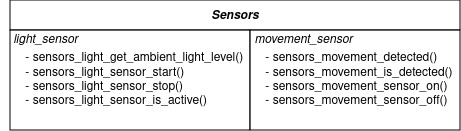
\includegraphics[scale=0.5]{./images/Sensors.jpg}
		\caption{Modulo Sensors}
		\label{img:sensors}
	\end{figure}
	\noindent Il modulo \textit{Sensors}, come evidenziato in precedenza, pu\`o essere considerato parte della componente per la gestione dell'illuminazione.
	
	\noindent Come si pu\`o notare in Figura \ref{img:sensors} il modulo presenta due sottomoduli:
	\begin{itemize}
			\item \textit{light\_sensor} che, tramite \texttt{ADC}, verifica il livello di luce ambientale.
			\item \textit{movement\_sensor} che permette di verificare la presenza di individui nelle vicinanze del sistema.
	\end{itemize}
	\newpage
	
	\subsubsection{Modulo Panic}
	\begin{figure}[ht]
		\centering
		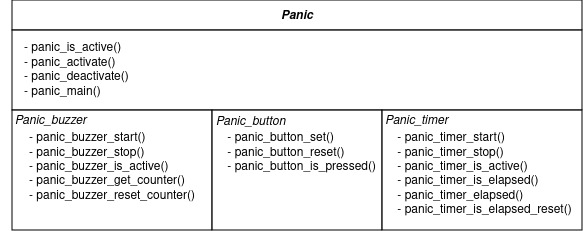
\includegraphics[scale=0.4]{./images/Panic.jpg}
		\caption{Modulo Panic}
		\label{img:panic}
	\end{figure}
	\noindent Il modulo \textit{Panic} rappresenta l'elemento software che gestisce per intero la componente per la segnalazione delle emergenze.
	Il modulo, come avviene all'interno delle altre componenti visibile anche in Figura \ref{img:panic}, presenta una serie di funzioni ad alto livello che fornisce tutte le funzioni necessarie per il funzionamento di base del componente.
	Sono presenti inoltre 3 sotto moduli, utilizzati direttamente dal modulo principale, che permettono di gestire singolarmente i vari elementi necessari:
	\begin{itemize}
		\item \textit{panic\_buzzer} che si occupa della gestione del buzzer per la generazione di segnali sonori.
		\item \textit{panic\_button} che gestisce le interazioni con il bottone di emergenza.
		\item \textit{panic\_timer} che utilizza il timer \texttt{TIM3} per gestire l'alternarsi di accensione e spegnimento del buzzer.
	\end{itemize}
	
	\subsubsection{Modulo Comm}
	\begin{figure}[ht]
		\centering
		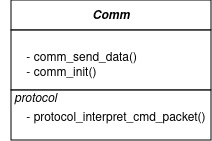
\includegraphics[scale=0.5]{./images/Comm.jpg}
		\caption{Modulo Comm}
		\label{img:comm}
	\end{figure}
	\noindent Il modulo \textit{Comm} rappresenta l'unico elemento della componente atta alla comunicazione con il coprocessore wireless.
	Il modulo in questione utilizza la comunicazione \texttt{uart} per inviare e ricevere i dati dal coprocessore.
	In particolare, l'invio dei dati, essendo un pacchetto periodico statico e avvendo con una frequenza abbastanza elevata(ogni 5 secondi), per non occupare inutilmente tempo CPU, utilizza il \texttt{DMA}.
	Per quanto riguarda la ricezione dei dati, invece, l'interfaccia \texttt{uart} viene utilizzata in modalit\`a \textit{interrupt}, in questo modo la reazione alla ricezione dei dati risulta essere immediata.
	Per poter interpretare correttamente i dati viene utilizzato il sottomodulo \textit{protocol} che fornisce la possibilit\`a di interpretare i comandi ricevuti dal router.
	
	\subsection{Coprocessore Wireless}
	Il componente hardware utilizzato come coprocessore wireless \`e un Raspberrypi Pico che utilizza il microprocessore \href{https://www.raspberrypi.com/documentation/microcontrollers/silicon.html#rp2040}{\textit{RP2040}}. Questo microprocessore presenta due core con architettura Arm-M0+.
	
	\noindent La presenza dei due core \`e stata sfruttata per implementare una suddivisione fisica, oltre che logica, dell'esecuzione dei due moduli presenti sul microcontrollore.
	L'architettura software presente sul coprocessore wireless \`e stata utilizzata anche all'interno del router, elemento atto all'invio dei dati e il controllo dello stato di funzionamento del sistema di illuminazione, sostituendo l'interfaccia di comunicazione seriale da \textit{uart} a \textit{usb}.
	
	\subsubsection{Modulo LoRa}
	Il modulo LoRa, utilizzato per la comunicazione radio, sfrutta la libreria \href{https://github.com/jgromes/RadioLib}{RadioLib} come driver per la gestione del LoRa shield collegato al Pico.
	Questo modulo utilizza invio e ricezione dei dati tramite interrupt che, come indicato all'interno della documentazione della libreria stessa, risulta essere il metodo pi\`u sicuro per evitare la perdita dei pacchetti.
	
	\subsubsection{Modulo Comm}
	\begin{figure}[ht]
		\centering
		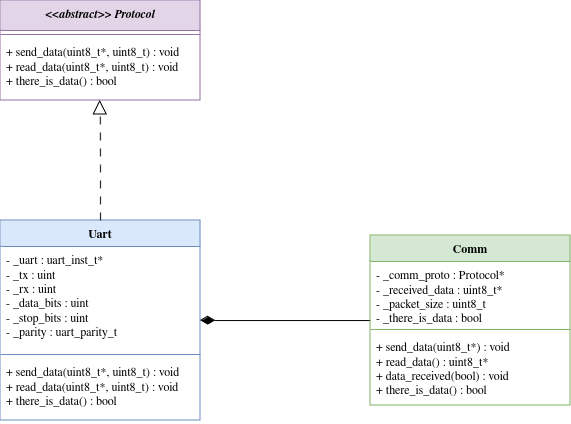
\includegraphics[scale=0.4]{./images/Comm_pico_uml.png}
		\caption{Modulo Comm del coprocessore}
		\label{img:comm_pico}
	\end{figure}
	\noindent Essendo la libreria utilizzata per la comunicazione wireless scritta interamente in \texttt{C++}, la libreria per la comunicazione seriale, come si pu\`o notare in Figura \ref{img:comm_pico} utilizza una gerarchie di classi per introdurre astrazione rispetto all'hardware sottostante.
	In particolare la libreria realizzata \textit{libcomm} presenta:
	\begin{itemize}
		\item la classe astratta \textit{Protocol}: la quale rappresenta l'insieme delle funzionalit\`a di base del protocollo di comunicazione seriale utilizzato.
		\item la classe \textit{Uart}: che implementa la classe \textit{Protocol} e fornisce il livello di astrazione rispetto l'interfaccia \textit{uart} utilizzata.
		\item la class \textit{Comm}: al cui interno \`e presente un puntatore ad una classe derivata da \textit{Protocol} che gestisce la comunicazione tenendo conto del protocollo di comunicazione utilizzato a livello dell'applicazione. Per la comunicazione dei vari dati, infatti, \`e stato definito un protocollo di comunicazione per racchiudere le varie informazioni nel minor numero di byte possibile.
	\end{itemize}
	Come detto anche in precedenza, l'unico elemento che distingue il funzionamento del coprocessore wireless rispetto al router risulta essere l'interfaccia seriale utilizzata. All'interno del router, infatti, la libreria \textit{libcomm} risulta essere uguale a quella presenta sul coprocessore con l'unica differenza che la classe utilizzata per implementare la classe astratta \textit{Protocol} risulta essere la classe \textit{Usb} che fornisce un'astrazione per quanto riguarda la comunicazione tramite la porta microusb presente sul Pico.
	
	\subsection{Protocollo di comunicazione}
	Il protocollo di comunicazione \`e stato pensato per avere un numero fisso di byte, ogni pacchetto infatti contiene esattamente quattro bytes.
	Il significato dei singoli byte risulta essere il seguente, come indicato in Figura \ref{img:}
	
	\subsection{Interazioni tra i moduli}
	

\end{document}